%% template.tex
%% from
%% bare_conf.tex
%% V1.4b
%% 2015/08/26
%% by Michael Shell
%% See:
%% http://www.michaelshell.org/
%% for current contact information.
%%
%% This is a skeleton file demonstrating the use of IEEEtran.cls
%% (requires IEEEtran.cls version 1.8b or later) with an IEEE
%% conference paper.
%%
%% Support sites:
%% http://www.michaelshell.org/tex/ieeetran/
%% http://www.ctan.org/pkg/ieeetran
%% and
%% http://www.ieee.org/

%%*************************************************************************
%% Legal Notice:
%% This code is offered as-is without any warranty either expressed or
%% implied; without even the implied warranty of MERCHANTABILITY or
%% FITNESS FOR A PARTICULAR PURPOSE!
%% User assumes all risk.
%% In no event shall the IEEE or any contributor to this code be liable for
%% any damages or losses, including, but not limited to, incidental,
%% consequential, or any other damages, resulting from the use or misuse
%% of any information contained here.
%%
%% All comments are the opinions of their respective authors and are not
%% necessarily endorsed by the IEEE.
%%
%% This work is distributed under the LaTeX Project Public License (LPPL)
%% ( http://www.latex-project.org/ ) version 1.3, and may be freely used,
%% distributed and modified. A copy of the LPPL, version 1.3, is included
%% in the base LaTeX documentation of all distributions of LaTeX released
%% 2003/12/01 or later.
%% Retain all contribution notices and credits.
%% ** Modified files should be clearly indicated as such, including  **
%% ** renaming them and changing author support contact information. **
%%*************************************************************************


% *** Authors should verify (and, if needed, correct) their LaTeX system  ***
% *** with the testflow diagnostic prior to trusting their LaTeX platform ***
% *** with production work. The IEEE's font choices and paper sizes can   ***
% *** trigger bugs that do not appear when using other class files.       ***                          ***
% The testflow support page is at:
% http://www.michaelshell.org/tex/testflow/

\documentclass[conference,final,]{IEEEtran}
% Some Computer Society conferences also require the compsoc mode option,
% but others use the standard conference format.
%
% If IEEEtran.cls has not been installed into the LaTeX system files,
% manually specify the path to it like:
% \documentclass[conference]{../sty/IEEEtran}





% Some very useful LaTeX packages include:
% (uncomment the ones you want to load)


% *** MISC UTILITY PACKAGES ***
%
%\usepackage{ifpdf}
% Heiko Oberdiek's ifpdf.sty is very useful if you need conditional
% compilation based on whether the output is pdf or dvi.
% usage:
% \ifpdf
%   % pdf code
% \else
%   % dvi code
% \fi
% The latest version of ifpdf.sty can be obtained from:
% http://www.ctan.org/pkg/ifpdf
% Also, note that IEEEtran.cls V1.7 and later provides a builtin
% \ifCLASSINFOpdf conditional that works the same way.
% When switching from latex to pdflatex and vice-versa, the compiler may
% have to be run twice to clear warning/error messages.






% *** CITATION PACKAGES ***
%
%\usepackage{cite}
% cite.sty was written by Donald Arseneau
% V1.6 and later of IEEEtran pre-defines the format of the cite.sty package
% \cite{} output to follow that of the IEEE. Loading the cite package will
% result in citation numbers being automatically sorted and properly
% "compressed/ranged". e.g., [1], [9], [2], [7], [5], [6] without using
% cite.sty will become [1], [2], [5]--[7], [9] using cite.sty. cite.sty's
% \cite will automatically add leading space, if needed. Use cite.sty's
% noadjust option (cite.sty V3.8 and later) if you want to turn this off
% such as if a citation ever needs to be enclosed in parenthesis.
% cite.sty is already installed on most LaTeX systems. Be sure and use
% version 5.0 (2009-03-20) and later if using hyperref.sty.
% The latest version can be obtained at:
% http://www.ctan.org/pkg/cite
% The documentation is contained in the cite.sty file itself.






% *** GRAPHICS RELATED PACKAGES ***
%
\ifCLASSINFOpdf
  % \usepackage[pdftex]{graphicx}
  % declare the path(s) where your graphic files are
  % \graphicspath{{../pdf/}{../jpeg/}}
  % and their extensions so you won't have to specify these with
  % every instance of \includegraphics
  % \DeclareGraphicsExtensions{.pdf,.jpeg,.png}
\else
  % or other class option (dvipsone, dvipdf, if not using dvips). graphicx
  % will default to the driver specified in the system graphics.cfg if no
  % driver is specified.
  % \usepackage[dvips]{graphicx}
  % declare the path(s) where your graphic files are
  % \graphicspath{{../eps/}}
  % and their extensions so you won't have to specify these with
  % every instance of \includegraphics
  % \DeclareGraphicsExtensions{.eps}
\fi
% graphicx was written by David Carlisle and Sebastian Rahtz. It is
% required if you want graphics, photos, etc. graphicx.sty is already
% installed on most LaTeX systems. The latest version and documentation
% can be obtained at:
% http://www.ctan.org/pkg/graphicx
% Another good source of documentation is "Using Imported Graphics in
% LaTeX2e" by Keith Reckdahl which can be found at:
% http://www.ctan.org/pkg/epslatex
%
% latex, and pdflatex in dvi mode, support graphics in encapsulated
% postscript (.eps) format. pdflatex in pdf mode supports graphics
% in .pdf, .jpeg, .png and .mps (metapost) formats. Users should ensure
% that all non-photo figures use a vector format (.eps, .pdf, .mps) and
% not a bitmapped formats (.jpeg, .png). The IEEE frowns on bitmapped formats
% which can result in "jaggedy"/blurry rendering of lines and letters as
% well as large increases in file sizes.
%
% You can find documentation about the pdfTeX application at:
% http://www.tug.org/applications/pdftex





% *** MATH PACKAGES ***
%
%\usepackage{amsmath}
% A popular package from the American Mathematical Society that provides
% many useful and powerful commands for dealing with mathematics.
%
% Note that the amsmath package sets \interdisplaylinepenalty to 10000
% thus preventing page breaks from occurring within multiline equations. Use:
%\interdisplaylinepenalty=2500
% after loading amsmath to restore such page breaks as IEEEtran.cls normally
% does. amsmath.sty is already installed on most LaTeX systems. The latest
% version and documentation can be obtained at:
% http://www.ctan.org/pkg/amsmath





% *** SPECIALIZED LIST PACKAGES ***
%
%\usepackage{algorithmic}
% algorithmic.sty was written by Peter Williams and Rogerio Brito.
% This package provides an algorithmic environment fo describing algorithms.
% You can use the algorithmic environment in-text or within a figure
% environment to provide for a floating algorithm. Do NOT use the algorithm
% floating environment provided by algorithm.sty (by the same authors) or
% algorithm2e.sty (by Christophe Fiorio) as the IEEE does not use dedicated
% algorithm float types and packages that provide these will not provide
% correct IEEE style captions. The latest version and documentation of
% algorithmic.sty can be obtained at:
% http://www.ctan.org/pkg/algorithms
% Also of interest may be the (relatively newer and more customizable)
% algorithmicx.sty package by Szasz Janos:
% http://www.ctan.org/pkg/algorithmicx




% *** ALIGNMENT PACKAGES ***
%
%\usepackage{array}
% Frank Mittelbach's and David Carlisle's array.sty patches and improves
% the standard LaTeX2e array and tabular environments to provide better
% appearance and additional user controls. As the default LaTeX2e table
% generation code is lacking to the point of almost being broken with
% respect to the quality of the end results, all users are strongly
% advised to use an enhanced (at the very least that provided by array.sty)
% set of table tools. array.sty is already installed on most systems. The
% latest version and documentation can be obtained at:
% http://www.ctan.org/pkg/array


% IEEEtran contains the IEEEeqnarray family of commands that can be used to
% generate multiline equations as well as matrices, tables, etc., of high
% quality.




% *** SUBFIGURE PACKAGES ***
%\ifCLASSOPTIONcompsoc
%  \usepackage[caption=false,font=normalsize,labelfont=sf,textfont=sf]{subfig}
%\else
%  \usepackage[caption=false,font=footnotesize]{subfig}
%\fi
% subfig.sty, written by Steven Douglas Cochran, is the modern replacement
% for subfigure.sty, the latter of which is no longer maintained and is
% incompatible with some LaTeX packages including fixltx2e. However,
% subfig.sty requires and automatically loads Axel Sommerfeldt's caption.sty
% which will override IEEEtran.cls' handling of captions and this will result
% in non-IEEE style figure/table captions. To prevent this problem, be sure
% and invoke subfig.sty's "caption=false" package option (available since
% subfig.sty version 1.3, 2005/06/28) as this is will preserve IEEEtran.cls
% handling of captions.
% Note that the Computer Society format requires a larger sans serif font
% than the serif footnote size font used in traditional IEEE formatting
% and thus the need to invoke different subfig.sty package options depending
% on whether compsoc mode has been enabled.
%
% The latest version and documentation of subfig.sty can be obtained at:
% http://www.ctan.org/pkg/subfig




% *** FLOAT PACKAGES ***
%

%\usepackage{fixltx2e}
% fixltx2e, the successor to the earlier fix2col.sty, was written by
% Frank Mittelbach and David Carlisle. This package corrects a few problems
% in the LaTeX2e kernel, the most notable of which is that in current
% LaTeX2e releases, the ordering of single and double column floats is not
% guaranteed to be preserved. Thus, an unpatched LaTeX2e can allow a
% single column figure to be placed prior to an earlier double column
% figure.
% Be aware that LaTeX2e kernels dated 2015 and later have fixltx2e.sty's
% corrections already built into the system in which case a warning will
% be issued if an attempt is made to load fixltx2e.sty as it is no longer
% needed.
% The latest version and documentation can be found at:
% http://www.ctan.org/pkg/fixltx2e


%\usepackage{stfloats}
% stfloats.sty was written by Sigitas Tolusis. This package gives LaTeX2e
% the ability to do double column floats at the bottom of the page as well
% as the top. (e.g., "\begin{figure*}[!b]" is not normally possible in
% LaTeX2e). It also provides a command:
%\fnbelowfloat
% to enable the placement of footnotes below bottom floats (the standard
% LaTeX2e kernel puts them above bottom floats). This is an invasive package
% which rewrites many portions of the LaTeX2e float routines. It may not work
% with other packages that modify the LaTeX2e float routines. The latest
% version and documentation can be obtained at:
% http://www.ctan.org/pkg/stfloats
% Do not use the stfloats baselinefloat ability as the IEEE does not allow
% \baselineskip to stretch. Authors submitting work to the IEEE should note
% that the IEEE rarely uses double column equations and that authors should try
% to avoid such use. Do not be tempted to use the cuted.sty or midfloat.sty
% packages (also by Sigitas Tolusis) as the IEEE does not format its papers in
% such ways.
% Do not attempt to use stfloats with fixltx2e as they are incompatible.
% Instead, use Morten Hogholm'a dblfloatfix which combines the features
% of both fixltx2e and stfloats:
%
% \usepackage{dblfloatfix}
% The latest version can be found at:
% http://www.ctan.org/pkg/dblfloatfix




% *** PDF, URL AND HYPERLINK PACKAGES ***
%
%\usepackage{url}
% url.sty was written by Donald Arseneau. It provides better support for
% handling and breaking URLs. url.sty is already installed on most LaTeX
% systems. The latest version and documentation can be obtained at:
% http://www.ctan.org/pkg/url
% Basically, \url{my_url_here}.




% *** Do not adjust lengths that control margins, column widths, etc. ***
% *** Do not use packages that alter fonts (such as pslatex).         ***
% There should be no need to do such things with IEEEtran.cls V1.6 and later.
% (Unless specifically asked to do so by the journal or conference you plan
% to submit to, of course. )



%% BEGIN MY ADDITIONS %%


\usepackage{graphicx}
% We will generate all images so they have a width \maxwidth. This means
% that they will get their normal width if they fit onto the page, but
% are scaled down if they would overflow the margins.
\makeatletter
\def\maxwidth{\ifdim\Gin@nat@width>\linewidth\linewidth
\else\Gin@nat@width\fi}
\makeatother
\let\Oldincludegraphics\includegraphics
\renewcommand{\includegraphics}[1]{\Oldincludegraphics[width=\maxwidth]{#1}}

\usepackage[unicode=true]{hyperref}

\hypersetup{
            pdftitle={An Experiment Comparing the Effectiveness of the Choropleth Map with a Hexagon Tile Map for Communicating Cancer Statistics},
            pdfkeywords={statistics, visual inference, geospatial, population},
            pdfborder={0 0 0},
            breaklinks=true}
\urlstyle{same}  % don't use monospace font for urls

% Pandoc toggle for numbering sections (defaults to be off)
\setcounter{secnumdepth}{0}

% Pandoc syntax highlighting

% Pandoc header
\usepackage{booktabs}
\usepackage{longtable}
\usepackage{array}
\usepackage{multirow}
\usepackage{wrapfig}
\usepackage{float}
\usepackage{colortbl}
\usepackage{pdflscape}
\usepackage{tabu}
\usepackage{threeparttable}
\usepackage{threeparttablex}
\usepackage[normalem]{ulem}
\usepackage{makecell}
\usepackage{xcolor}

\providecommand{\tightlist}{%
  \setlength{\itemsep}{0pt}\setlength{\parskip}{0pt}}

%% END MY ADDITIONS %%


\hyphenation{op-tical net-works semi-conduc-tor}

\begin{document}
%
% paper title
% Titles are generally capitalized except for words such as a, an, and, as,
% at, but, by, for, in, nor, of, on, or, the, to and up, which are usually
% not capitalized unless they are the first or last word of the title.
% Linebreaks \\ can be used within to get better formatting as desired.
% Do not put math or special symbols in the title.
\title{An Experiment Comparing the Effectiveness of the Choropleth Map with a
Hexagon Tile Map for Communicating Cancer Statistics}

% author names and affiliations
% use a multiple column layout for up to three different
% affiliations

\author{

%% ---- classic IEEETrans wide authors' list ----------------
 % -- end affiliation.wide
%% ----------------------------------------------------------



%% ---- classic IEEETrans one column per institution --------
 %% -- end if/affiliation.institution-columnar
%% ----------------------------------------------------------





%% ---- one column per author, classic/default IEEETrans ----
 % -- beg affiliation.author-columnar
  %% -- beg for/affiliation.institution.author
\IEEEauthorblockN{
Stephanie Kobakian
}
\IEEEauthorblockA{Queensland University of Technology\\
Science and Engineering Faculty\\
Brisbane, Australia
\\stephanie.kobakian@qut.edu.au
}
 %% -- end for/affiliation.institution.author
\and
  %% -- beg for/affiliation.institution.author
\IEEEauthorblockN{
Dianne Cook
}
\IEEEauthorblockA{Monash University\\
Econometrics and Business Statistics Faculty\\
Melbourne, Australia
\\dicook@monash.edu
}
 %% -- end for/affiliation.institution.author
 %% -- end for/affiliation.institution
 %% -- end if/affiliation.institution-columnar
%% ----------------------------------------------------------

}

% conference papers do not typically use \thanks and this command
% is locked out in conference mode. If really needed, such as for
% the acknowledgment of grants, issue a \IEEEoverridecommandlockouts
% after \documentclass

% for over three affiliations, or if they all won't fit within the width
% of the page, use this alternative format:
%
%\author{\IEEEauthorblockN{Michael Shell\IEEEauthorrefmark{1},
%Homer Simpson\IEEEauthorrefmark{2},
%James Kirk\IEEEauthorrefmark{3},
%Montgomery Scott\IEEEauthorrefmark{3} and
%Eldon Tyrell\IEEEauthorrefmark{4}}
%\IEEEauthorblockA{\IEEEauthorrefmark{1}School of Electrical and Computer Engineering\\
%Georgia Institute of Technology,
%Atlanta, Georgia 30332--0250\\ Email: see http://www.michaelshell.org/contact.html}
%\IEEEauthorblockA{\IEEEauthorrefmark{2}Twentieth Century Fox, Springfield, USA\\
%Email: homer@thesimpsons.com}
%\IEEEauthorblockA{\IEEEauthorrefmark{3}Starfleet Academy, San Francisco, California 96678-2391\\
%Telephone: (800) 555--1212, Fax: (888) 555--1212}
%\IEEEauthorblockA{\IEEEauthorrefmark{4}Tyrell Inc., 123 Replicant Street, Los Angeles, California 90210--4321}}




% use for special paper notices
%\IEEEspecialpapernotice{(Invited Paper)}




% make the title area
\maketitle

% As a general rule, do not put math, special symbols or citations
% in the abstract
\begin{abstract}
Choosing a visualisation method may seem to be a simple task. The
choropleth map display is commonly used for communicating spatial data.
However, when used to communicate the spatial distribution of a
statistic the sizes of areas can lead to midinterpretation of the
distribution. The visualisation method used to present geospatial data
will influence the information derived by map users. Choosing an
alternative display will influence the communication of the
distribution. The hexagon tile map is presented as an alternative
display. Visual inference is used to measure the power of design. The
choropleth is used as a comparison point. The hexagon tile map display
is an effective visualisation for communicatin=g population related
distributions. The hexagon tile map display also allowed identification
of the geographic distribution with values monotonically decreasing from
North West toward South East areas of Australia.
\end{abstract}

% keywords
\begin{IEEEkeywords}
statistics; visual inference; geospatial; population
\end{IEEEkeywords}

% use for special paper notices



% make the title area
\maketitle

% no keywords

% For peer review papers, you can put extra information on the cover
% page as needed:
% \ifCLASSOPTIONpeerreview
% \begin{center} \bfseries EDICS Category: 3-BBND \end{center}
% \fi
%
% For peerreview papers, this IEEEtran command inserts a page break and
% creates the second title. It will be ignored for other modes.
\IEEEpeerreviewmaketitle


\hypertarget{introduction}{%
\section{Introduction}\label{introduction}}

This study contrasts the use of two displays for geospatial statistics,
the traditional choropleth map and an alternative tessellated hexagon
tile map. The choropleth map is the common choice for visualising
aggregated statistics and is familiar because of common administrative
boundaries. A hexagon tile map forgoes the familiar boundaries, instead
representing each geographic unit as an equally sized hexagon. This
alternative display is suggested for communicating distributions that
relate to the population values or density of the population in each
geographic unit. This study uses the lineup protocol for visual
inference testing of the recognition of spatial distributions. The
Australian Cancer Atlas explores spatial distributions of cancer
incidence and the burden on Australian communities. The spatial
distributions of the cancers explored in this atlas inspired the trend
models presented to participants in this study.

\hypertarget{motivation}{%
\section{Motivation}\label{motivation}}

\hypertarget{the-australian-cancer-atlas}{%
\subsection{The Australian Cancer
Atlas}\label{the-australian-cancer-atlas}}

The Australian Cancer Atlas is an online interactive web tool created to
explore the burden of cancer on Australian communities. There are many
cancer types to be explored individually or aggregated. The Atlas
examines Australian communities at the Statistical Areas at Level 2
(SA2) (``Australian Statistical Geography Standard (ASGS)''
\protect\hyperlink{ref-abs2016}{2018}) used by the Australian Bureau of
Statistics. Bayesian spatial smoothing was applied to integrate the
values of neighbouring areas. Spatial smoothing protects the privacy and
gives stability to the estimated amounts in each SA2. Users of the Atlas
can explore the difference of the statistic of each SA2 from the
Australian average, for both diagnoses (Standardised Incidence Rates)
and excess deaths. It communicates the value of the statistic for each
SA2 geographic unit through colour, by filling the areas using the
diverging colour scheme ranging from dark blue to red. The Australian
Cancer Atlas allows users to explore the patterns in the distributions
of cancer statistics over the geographic space of Australia. It uses a
choropleth map display and diverging colour scheme to draw attention to
relationships between neighbouring areas.

\hypertarget{background}{%
\section{Background}\label{background}}

\hypertarget{population-focussed-displays}{%
\subsection{Population focussed
displays}\label{population-focussed-displays}}

Spatial visualisations communicate the distribution of statistics over
geographic space. The most common display for spatial data is the
choropleth map. The choropleth map is the common display used to present
aggregated statistics for geographic units such as the population.
Creating a choropleth map involves drawing the administrative boundaries
and filling them with colour to communicate the value of the statistic.
However, using a choropleth map base introduces biases when considering
population related distributions. Many sets of Australian statistical
areas have a large disparity between the smallest and largest units. The
rural communities in Australia operate on a much larger geographic space
than small inner-city communities. When a spatial distribution is
related to the size of the areas, or the population density, the size of
the regions can allow erroneous conclusions to be drawn about the state
of the statistic over the entire population, when presenting the
statistics on a geographic map base. This occurs as large regions filled
with a consistent colour or pattern can draw the attention of map
readers, and small regions are not paid equal attention. An alternative
display can be used to effectively communicate a spatial distribution
for a set of heterogeneous areas. This work aims to show that a hexagon
tile map display is a viable alternative to the geographic map base for
presenting population statistics.

A choropleth map is not the only display that can be used for presenting
geospatial data. Alternative maps include various cartograms and
tessellated tile maps. They allow other variables to be incorporated in
the display to highlight the statistical values of various geographic
areas.

A cartogram transforms the geographic map base. The transformation
begins with a choropleth map, and the values of a statistic such as
population, for each geographic unit. There are several algorithms for
transformation; they involve shifting the boundaries of geographic
units, using the value of the statistic to increase or decrease the area
taken by the geographic unit on the map. The changes to the boundaries
result in cartograms that accurately communicate population by map area
for each of the geographic units. The transformation will keep
boundaries of neighbouring areas connected, but the result is unfamiliar
shapes for each geographic unit.

Alternative displays make the trade off between familiar shapes and
representation of variables using the area of geographic units. The
non-contiguous cartgoram method keeps the shapes of geographic units
intact, and change the size of the shape to communicate the values of
statistics. This method disconnects areas when shrinking boundaries, and
breaks the spatial relationship between areas. However, the empty space
created emphasises the comparative density of the statistic, the
difference between the statistic and the amount of land for each
geographic unit. The Dorling cartogram is another method that does not
retain the boundaries of geographic units. Each unit becomes one circle
on the cartogram display; the circles are sized according to the value
of a the statistic, such as population. The neighbour relationships can
be illustrated by connecting the boundaries of the circles. These
cartogram methods all allow two variables to be shown in the single
display.

\begin{figure}
\centering
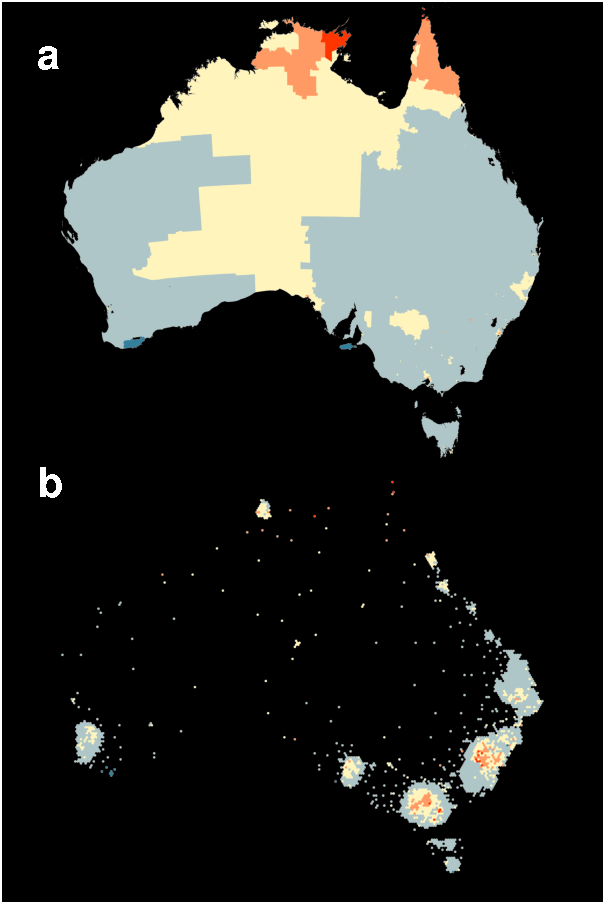
\includegraphics{paper_files/figure-latex/liver-1.pdf}
\caption{The smoothed average of liver cancer diagnoses for Australian
males. The divering colour scheme shows dark blue areas with much lower
than average diagnoses, yellow areas with diagnoses around the
Australian average, orange with above average and red shows diagnoses
much higher than average.}
\end{figure}

Australia is an extreme case of heterogenous geographic units, with
large difference between the smallest and largest geographic units
across various granularities. To communicate information regarding the
small inner-city geographic units of Australian cities an alternative
display must be employed. This will emphasise the value of the statistic
for areas with high population. Figure @ref(fig:liver) shows the
distribution of the smoothed average amount of Liver cancer diagnoses
for Australian Males from 2005-2014. These inner-city areas are not
visible on the choropleth map (a). The hexagon tile map (b) shows orange
hexagons for the inner-city SA2s with higher than average levels of
diagnoses in the capital cities of Melbourne and Sydney. The northern
Queensland, and Northern Territory SA2's with higher than average rates
are still visible but use less map space on the hexagon tile map. There
are still many light blue areas in both displays.

\hypertarget{visual-inference}{%
\subsection{Visual Inference}\label{visual-inference}}

The hexagon tile map is suggested as an alternative display. To test the
effectiveness of these displays there is a formal testing framework.
Visual inference considers the communication of data or data summaries
through visualisations. It considers these visualisations to be visual
statistics, with observable features.

Classical statistical inference involves hypothesis testing, the process
of rejecting a null hypothesis in favour of an alternative. This
approach requires appropriate data, with the appropriate distributions
and their assumptions. The lineup protocol was formalised as a test for
the effectiveness of a visualisation. Rather than use classical
statistical tests, human participants are tasked with finding the
display that shows structure between the variables. If the structure is
not detected, then it is not significantly different from the null data.

Visual inference uses the general hypothesis structure:

Null hypothesis: There is NO relationship between the variables,
Alternative hypothesis: There is a relationship between the variables.

To test these hypotheses, the line up protocol randomly places a
``guilty'' data visualisation in a lineup of ``innocents''. Where the
guilty data set contains structure, and the innocents data sets do not.
In a grid of visualisations, an observer is asked to pick the display
that is most different, if they select the data set containing
structure, they have identified the guilty hidden within the innocents
(Hofmann et al. \protect\hyperlink{ref-GTPCCD}{2012}). The guilty data
is identified as different from the innocent data with probability
\(1/m\), where \(m\) is the number of null plots plus 1 to account
account for the guilty data set. When the guilty data set is chosen, the
null hypothesis that it was innocent is rejected with a \(1/m\) chance
or type I error of being wrong.

The lineup protocol can be used in a variety of testing scenarios for
visualisations. Wickham et al. (\protect\hyperlink{ref-GIIV}{2010})
suggest the choropleth map for testing spatial structure in a data set.
The lineup protocol allows for flexibility in the definition of null
data. In the case of spatial visualisations it is likely that neighbours
are related to some degree. To account for this, null data sets can be
generated by sampling from a known model that accounts for spatial
covariance.

To contrast the effectiveness of two displays, the data set of null data
plots with a hidden real data plot can be produced using the different
plot designs. The time taken by participants to evaluate the same data
in the different displays can be compared. Their accuracy in detecting
the real data plot can also be calculated and contrasted.

\hypertarget{methodology}{%
\section{Methodology}\label{methodology}}

This study aimed to answer two key questions around the presentation of
spatial distributions:

\begin{enumerate}
\def\labelenumi{\arabic{enumi}.}
\item
  Are spatial disease trends, that impact highly populated small areas,
  detected with higher accuracy when viewed in a hexagon tile map
  display?
\item
  Are people faster in detecting spatial disease trends, that impact
  highly populated small areas, when using a hexagon tile map display?
\end{enumerate}

Additional considerations when completing this experimental task
included exploration of the difficulty experienced by participants, and
the certainty they felt about their decision.

The mean of the detection rate for choropleth map, denoted as \(\mu_C\),
and the hexagon tile maps, \(\mu_H\) will be contrasted. This leads to
the following one sided hypothesis:

\(H_0\) : \(\mu_H\) = \(\mu_C\) \(H_a\) : \(\mu_H\) \textgreater{}
\(\mu_C\)

The detection rate \(\hat\pi\) is calculated as the amount of people
that made the choice of plot that contained the real data, out of the
participants who saw data plot in the lineup of the null data plots.

The difference in the detection rates for the two displays will be
compared using a two sample unpaired t-test.

\hypertarget{participants}{%
\subsection{Participants}\label{participants}}

Participants were recruited for a survey style task to test the
effectiveness of the hexagon tile map display. It was expected that the
participants were uninvolved judges that had no prior knowledge of the
data, to avoid discrimination or advantages. The Figure-Eight crowd
source platform was used to advertise the survey to potential
participants that had acheived level 2 or level 3 on the Figure-Eight
Platform. The participants were chosen as they have experience with
survey tasks that involve evaluating images. They participants on the
platform are also required to be at least 18 years old.

Participants were able to choose to participate by selecting this task
from the list of tasks available to them. There were 95 participants
involved in the study. All of these participants read the introductory
materials and viewed example questions before proceeding to the survey.
Each participant was trained using three test displays orienting them to
the evaluation task, these displays are shown in supplementary materials
section regarding \protect\hyperlink{training}{training}. All
participants who volunteered to take part were compensated for their
time via the payment system of Figure-Eight.

Participants were allocated to either group A or group B when they
proceeded to the survey web application, hosted externally from the
Figure-Eight website.

\hypertarget{variables}{%
\subsection{Variables}\label{variables}}

The variables that were changed between groups were the type of plot
shown and the trend model.

The twenty-four lineup displays were created by a combination of map
type, and spatial trend model. This set of displays was split into a
collection of twelve displays for Group A and twelve displays for Group
B.

Each participant was randomly allocated to either Group A or Group B
when they begun the survey. This resulted in 42 participants allocated
to Group A, and 53 participants allocated to Group B.

The levels of the factors measured in the experiment were:

\begin{itemize}
\tightlist
\item
  Map type: \emph{Choropleth, Hexagon tile}
\item
  Trend: \emph{Locations in three population centres, Locations in
  multiple population centres, South-East to North-West}
\end{itemize}

Each Group did not see the same data for both map types. Four simulated
sets of data were generated for each treatment. This will generate
twenty-four lineups (twelve lineups of geographic maps, and twelve
lineups of hexagon tile maps). Participants evaluated twelve lineups,
siz of each map type. For each of the six geographic displays and six
hexagon displays, two of each trend model were shown to participants.

\begin{table}

\caption{\label{tab:exp_design}Experimental design.}
\centering
\begin{tabular}[t]{llll}
\toprule
Group & Trend & Choro. & Hex.\\
\midrule
A & NW-SE & 1, 2 & 3, 4\\
A & Three Cities & 1, 2 & 3, 4\\
A & All Cities & 2, 4 & 1, 3\\
B & NW-SE & 3, 4 & 1, 2\\
B & Three Cities & 3, 4 & 1, 2\\
\addlinespace
B & All Cities & 1, 3 & 2, 4\\
\bottomrule
\end{tabular}
\end{table}

The variables measured as a result of the changes were the probability
of detection each display and the time taken to submit responses. To
measure the accuracy of the detections, the plot chosen for each lineup
evaluated was compared to the position of the real spatial trend plot in
the lineup. A correct result occurs when the chosen plot matches the
position of the real plot, this was recorded in an additional binary
variable; 1 = correct; 0 = incorrect. High efficiency occurs when a
small amount of time is taken to evaluate each lineup. This will be
measured as the numeric variable measuring the length of time taken to
submit the answers to the evaluation of each line up.

\hypertarget{simulation-process}{%
\subsection{Simulation process}\label{simulation-process}}

The lineup protocol allows a known model to be imposed on the null data
set plots. The underlying spatial correlation model was created to
provide spatial autocorrelation between neighbouring areas using the
longitude and latitude values for the Statistical Areas.

\[z = 1\] \[locations = longitude + latitude\]

The null model imposed suggests that neighbours are related. The
randomness imposed was smoothed to mirror the practice taken by the
Australian Cancer Atlas. This smoothing allowed neighbours to be related
to each other and show distributions similar to the Liver cancer
distribution shown in @ref(fig:liver).

Spatially dependent data sets were simulated using the variogram model
on the centroids of each geographic unit. Twelve simulations from the
variogram model were created for each of the twelve lineups.

In these 12 sets of data, each of the 144 maps were smoothed several
times to replicate the spatial autocorrelation seen in cancer data sets
presented in the Australian Cancer Atlas.

For each of the 144 individual maps, the values attributed to each
geographic area are rescaled to show a similar colour scale from deep
blue to dark red within each map.

A random location was selected for each set of lineup data. In this
location, a trend model was overlaid on the null set of spatially
correlated data. Each set of lineup data was used to produce a
choropleth maps and hexagon tile maps. These matched pairs were split
between Group A and Group B.

Replicate 3 of the All Cities distribution is shown in
@ref(fig:compare). The same data set is shown in both displays, the
difference is the land area of each SA3 is coloured in the choropleth
and the hexagon representing the SA3 is coloured in the Hexagon Tile
Map. Many maps in the Choropleth lineup (a) are coloured yellow, two are
half light blue, and two are obviously blue. Only one of the maps looks
red.

\begin{figure}
\centering
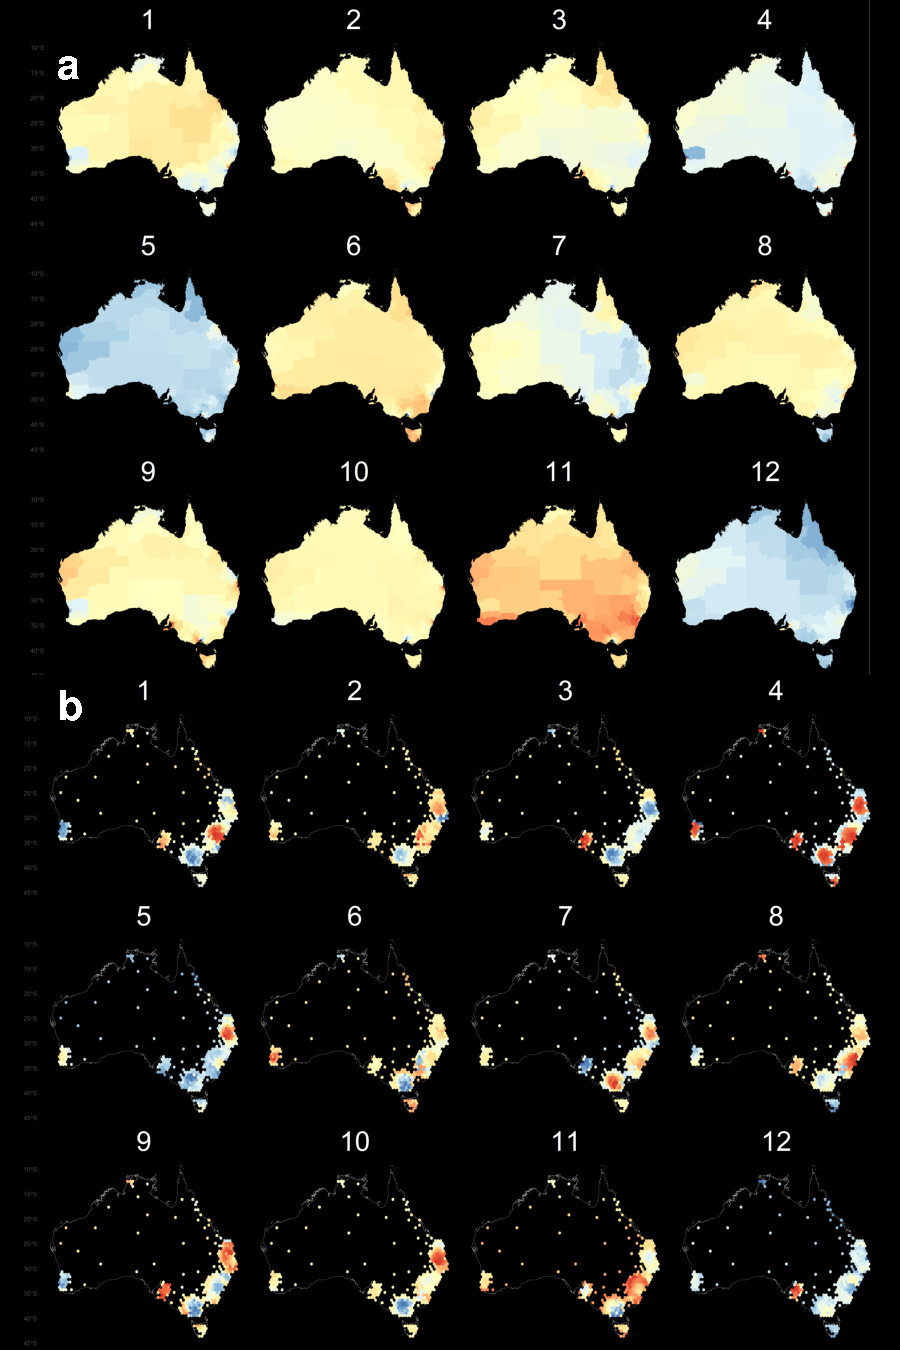
\includegraphics{paper_files/figure-latex/compare-1.pdf}
\caption{Comparing the same data presented in two map displays. The
choropleth map display in (a)}
\end{figure}

\hypertarget{experiment-procudure-and-data-collection}{%
\subsection{Experiment procudure and data
collection}\label{experiment-procudure-and-data-collection}}

The participant answered demographic questions and provided consent
before evaluating the lineups.

Demographics were collected regarding the study participants: - Gender
(female / male / other), - Degree education level achieved (high school
/ bachelors / masters / doctorate / other), - Age range (18-24 / 25-34 /
35-44 / 45-54 / 55+ / other) - Lived at least for one year in Australia
(Yes / No )

Participants then moved to the evaulation phase. The set of images
differed for Group A and Group B. After being allocated to a group, each
individual was shown the 12 displays in randomised order.

Three questions were asked regarding each display: - Plot choice -
Reason - Difficulty

After completing the 12 evaluations, the participants were asked to
submit their responses.

Data was collected through a web application containing the online
survey. Each participant used the internet to access the survey. The
data collection took place using a secure link between the survey web
application and the googlesheet used to store results. The application
would first connect to the googlesheet using the googlesheets (Bryan and
Zhao \protect\hyperlink{ref-sheets}{2018}) R package, and interacted
again at the completion of the survey by adding the participant's
responses to the 12 displays as 12 rows of data in the googlesheet.

\hypertarget{experimental-design}{%
\subsection{Experimental design}\label{experimental-design}}

The choropleth map was used as the comparative visualisation for
presenting the lineups (Majumder, Hofmann, and Cook
\protect\hyperlink{ref-VVSIALM}{2013}) as this is the common display for
spatial cancer data. Geographic distributions usually have some degree
of spatial autcorrelation between neighbours. This feature was
incorporated in all maps shown in the lineup displays, the map that
contained the trend feature shown in only one set of data was also
affected by spatial autocorrelation. A line up protocol was implemented
to arrange \(N\) maps in each display. A reasonable amount of null plots
\(N-1\) in the lineup was chosen to ensure the real data map was well
hidden. A reasonable number of plots to show in each lineup, \(N = 12\)
was chosen to not overwhelm participants due to the detailed choropleth
maps of Australian SA3 areas.

The hypotheses for each lineup are \(H_0\) : All plots look the same
\(H_a\) : One plot looks different to the other plots

The same data was visualised on a choropleth map, and on a hexagon tile
map, however in this study the participants only saw one of these two
displays. The accuracy and times taken were aggregated for Groups and.
Comparing the results of participants who see the choropleth to those
who see a hexagon tile map will show that population related
distributions are spotted more frequently in a hexagon tile map display.

Let \(n\) be the number of independent observers and \(x_i\) the number
of observers who picked plot \(i\), \(i = \{1,...,m\}\)

Then \(x_i, x_2, ..., x_m\) follows a multinomial
distribution\(Mult_{\pi_1, \pi_2, ...., \pi_m}(x_i, x_2, ..., x_m)\)
with \(\sum_i \pi_i = 1\), where \(\pi_i\) is the probability that plot
\(i\) is picked by an observer, which we can estimate as
\(\hat{\pi}_i = x_i/n\). The researchers compared the length of time
taken, and the accuracy of the participants choices. The power of a
lineup can therefore be estimated as the ratio of correct
identifications \(x\) out of \(n\) viewings.

\hypertarget{the-methods-of-data-analysis-used}{%
\subsection{The methods of data analysis
used}\label{the-methods-of-data-analysis-used}}

The data analysis methods used in order to analyse and collate the
results included downloading the survey submissions and opening them
into the analysis software R (R Core Team
\protect\hyperlink{ref-RCore}{2019}).

For each of the 12 lineup displays the researchers calculated: -
accuracy: the proportion of subjects who detected the data plot -
efficiency: average time taken to respond

\hypertarget{visualisations}{%
\subsubsection{Visualisations}\label{visualisations}}

Side-by-side dot plots were made of accuracy (efficiency) against map
type, facetted by trend model type.

Similar plots were made of the feedback and demographic variables -
reason for choice, reported difficulty, gender, age, education, having
lived in Australia - against the design variables.

Plots will be made in R (R Core Team 2019), with the ggplot2 package
(Wickham 2016).

\hypertarget{modeling}{%
\subsubsection{Modeling}\label{modeling}}

The results will be analysed using a generalised linear model, with a
subject random effect to account for differences in individuals. There
will be two main effects: map type and trend model, which gives the
fixed effects part of the model to be

\[\widehat{y_{ij}} = \mu + \tau_i + \delta_j + (\tau\delta)_{ij}, ~~~ i=1,2; ~j=1,2,3\]

where \(y_{ij} = 0, 1\) whether the subject detected the data plot,
\(\mu\) is the overall mean, \(\tau_i, i=1,2\) is the map type effect,
\(\delta_j\) is the trend model effect. We are allowing for an
interaction between map type and trend model. As the response for
whether the participant detected the data plot is binary, a logistic
model is used.

A similar model will be constructed for the efficiency, using a log
time, and normal errors.

The feedback and demographic variables will possibly be incorporated as
covariates.

Computation will be done using R (R Core Team
\protect\hyperlink{ref-RCore}{2019}), with the \texttt{lme4} package
(Bates et al. \protect\hyperlink{ref-lme4}{2015}).

\hypertarget{limitations-of-the-data-collection}{%
\subsection{Limitations of the data
collection}\label{limitations-of-the-data-collection}}

A pilot study was conducted to determine whether the lineups were
appropriate. All lineups in the pilot study were deemed viable as at
least one participant detected the real data plot in each lineup. The
demographics of the participants showed a skew towards male
participants. The randomness of the group allocation also resulted in
more participants being allocated to Group B. Due to the allocation of
lineup displays the participants all saw six Choropleth displays and six
Hexagon Tile Map displays.

\hypertarget{results}{%
\section{Results}\label{results}}

Responses from 95 participants were collected. Three participants
provided no answers for any task, and their data was removed. Set A was
evaluated by 42 participants, and 53 evaluated set B. This resulted in
1104 evaluations, corresponding to 92 subjects, each evaluating 12
lineups, that are analysed on accuracy and speed.

\hypertarget{participant-demographics}{%
\subsection{Participant demographics}\label{participant-demographics}}

Of the 92 participants, 67 were male, and 25 female. Most participants
(56) had a Bacherlors degree, 13 had a Masters degree, and the remaining
23 had high school diplomas.

\hypertarget{accuracy}{%
\subsection{Accuracy}\label{accuracy}}

Figure @ref\{detection\_compare\} display the average detection rates by
type of plot, separately for each trend model. Evaluations on the same
data set are connected by a line segment. For both the Three Cities and
All Cities trend models performance was substantially better for the
hexagon tile map. Viewers detected the data plot substantially more
often with the hexagon tile map. One replicate for the All Cities group,
had similar detection rates for both plot types, and this is discussed
in a later section. Surprisingly, participants could also detect the
gradual spatial trend in the NW-SE group from the hexagon tile map. We
expected that the choropleth map would be superior for the type of
spatial pattern, but the data suggests the hexagon tile map performs
equally as well.

Table \ref{tab:desc_stats} shows the means and standard deviations for
type of plot and each trend model.

\begin{figure}
\centering
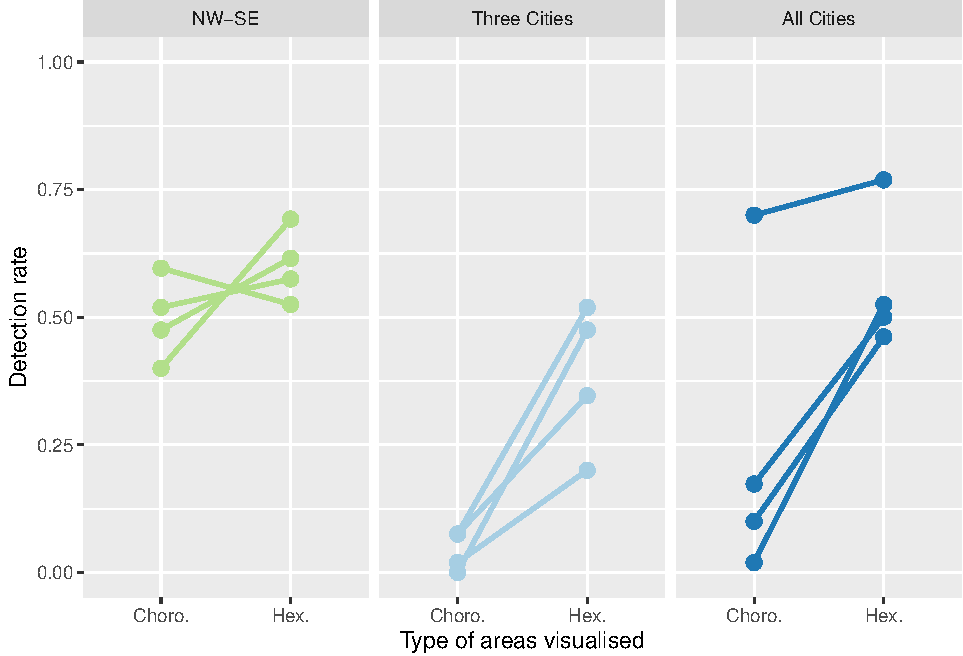
\includegraphics{paper_files/figure-latex/detection_compare-1.pdf}
\caption{The detection rates achieved by participants are contrasted
when viewing the four replicates of the three trend models. Each point
shows the probability of detection for the lineup display, the facets
separate the trend models hidden in the lineup. The points for the same
data set shown in a choroleth or haxgon tile map display are linked to
show the difference in the detection rate.}
\end{figure}

\begin{table}

\caption{\label{tab:desc_stats}}
\centering
\begin{tabular}[t]{lccc}
\toprule
Type & NW-SE & Three Cities & All Cities\\
\midrule
Choro. & 0.505 & 0.038 & 0.228\\
 & (0.5) & (0.19) & (0.42)\\
Hex. & 0.609 & 0.391 & 0.571\\
 & (0.49) & (0.49) & (0.5)\\
\bottomrule
\end{tabular}
\end{table}

Table XXX is a summary of the mixed effects model. Blah, blah, what we
learn.

\hypertarget{speed}{%
\subsection{Speed}\label{speed}}

The amount of time taken for a participants to submit a response is
explored. The time considered was the amount of time it took for a
participant to submit their choice of plot, the reason for their choice,
and the perceived difficulty of the choice. The time was taken when each
participant hit ``Next''.

The relationship between time taken to submit, and the correct detection
by the participant of the real data display in a lineup is considered in
Figure @ref(fig:hist\_height). The bimodal distributions are similar
across the type of display and the trend model hidden in the real data
plot. The hexagon map displays have a peak for the group that took up to
5 seconds to submit a response. When viewing a choropleth map display,
the second peak occured at around 20 seconds. The longest a participant
took to respond was 60 seconds.

\begin{figure}
\centering
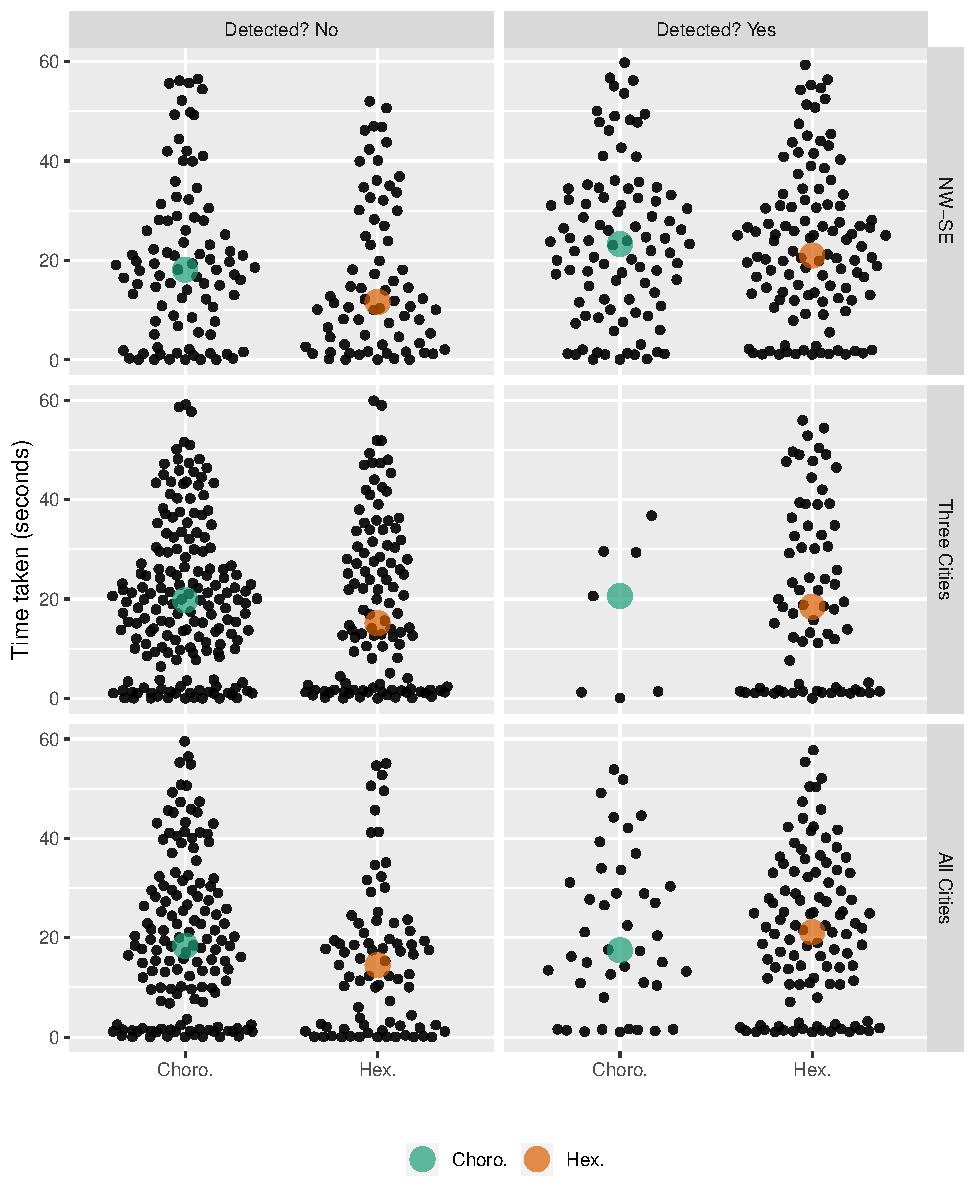
\includegraphics{paper_files/figure-latex/beeswarm-1.pdf}
\caption{The beeswarm plots show the distribution of the time taken to
submit a response for each combination of trend and type of display. The
time taken shown by the height of the point for each evaluationq1. The
height of the histogram bars show how many evaulations were submitted
within each time window. The orange regions of the bars show the amount
of correct detections, and the green regions are the amount of incorrect
detections.}
\end{figure}

The proportion of correct and incorrect responsesis shown by the width
used to distribute the points horizontally. Each point is randomly
placed, but regions with more points require points to be placed further
from center. For the NW-SE distribution, it is equally likely that quick
responders will be correct or incorrect. It is more likely that
participants picked the correct response if they took longer to respond.
For the Choropelth

However, these quick responders were likely to be either correct or
incorrect. The quick responders viewing a choropleth display were
unlikely to choose correctly, unless viewing a NW-SE trend model.

The choropleth map displays that included a distribution of three cities
was very difficult for participants.

\hypertarget{certainty}{%
\subsection{Certainty}\label{certainty}}

\begin{figure}
\centering
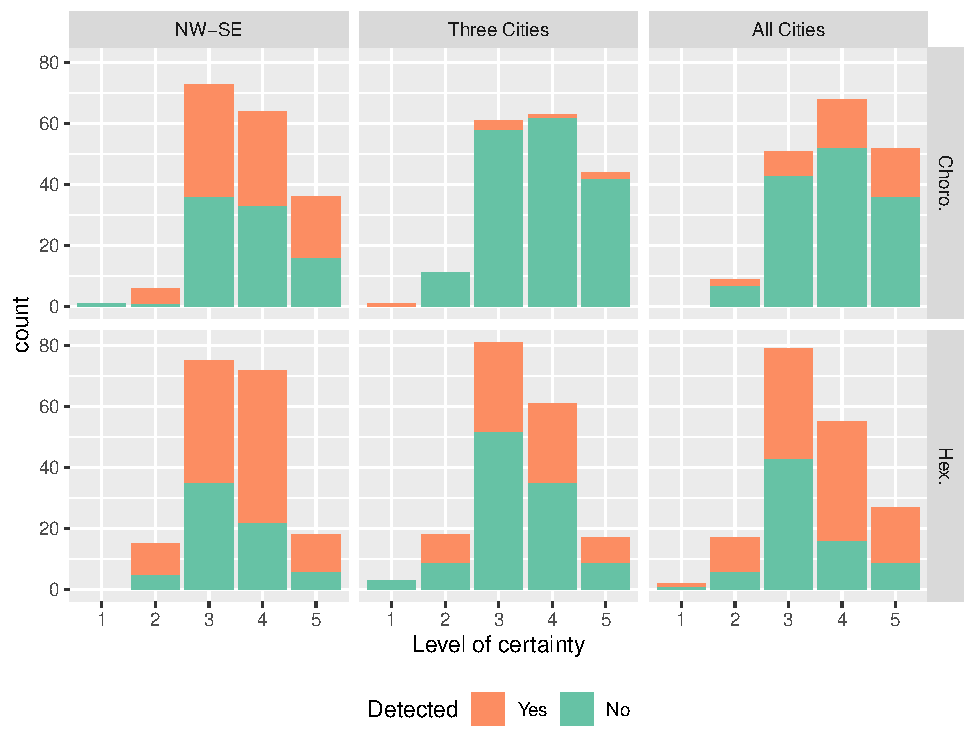
\includegraphics{paper_files/figure-latex/certainty-1.pdf}
\caption{The amount of times each level of certainty was chosen by
participants when viewing hexagon tile map or choropleth displays.
Participants were more likely to choose a high certainty when
considering a Choropleth map. The mid value of 3 was the default
certainty, it was chosen most for the Hexagon tile map displays.}
\end{figure}

Certainty levels are measured on a five point scale---they are
subjective assessments by the participant `How certain are you about
your choice?'.

\hypertarget{reason}{%
\subsection{Reason}\label{reason}}

\begin{table}[H]
\centering
\begin{tabular}{llll}
\toprule
Trend & Detected & Choro. & Hex.\\
\midrule
NW-SE & No & trend & clusters\\
NW-SE & Yes & trend & clusters\\
Three Cities & No & trend & clusters\\
Three Cities & Yes & consistent & clusters\\
All Cities & No & trend & clusters\\
\addlinespace
All Cities & Yes & clusters, consistent & clusters\\
\bottomrule
\end{tabular}
\end{table}

The most common choice made by participant was clusters, this response
was expected when participants viewed the Hexagon display of the all
cities and three cities distributions.

\hypertarget{contributors}{%
\subsection{Contributors}\label{contributors}}

\begin{figure}
\centering
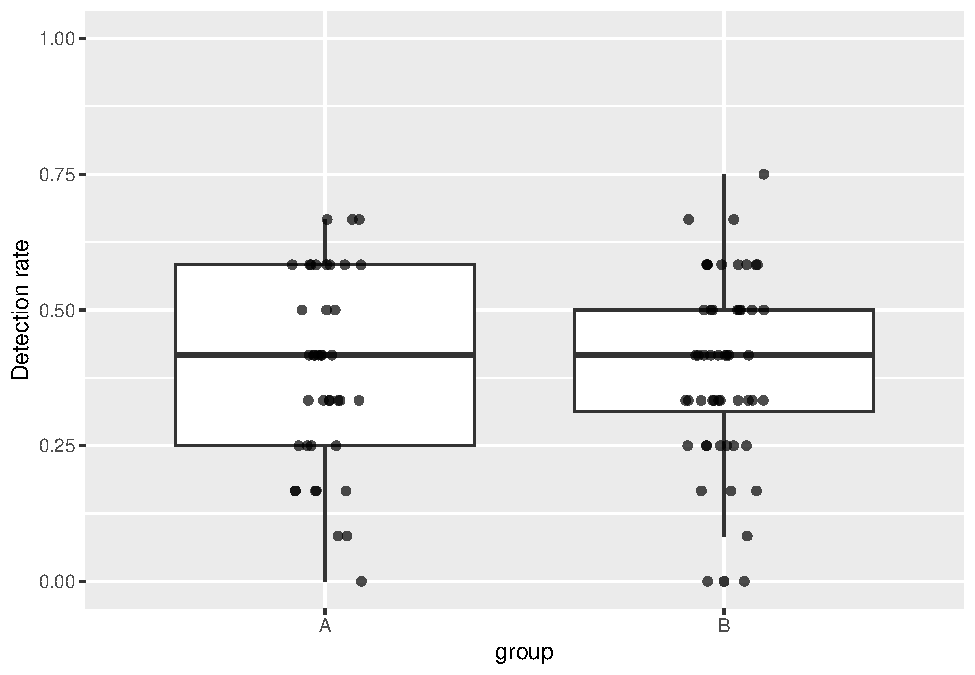
\includegraphics{paper_files/figure-latex/contributors-1.pdf}
\caption{The probablity of detection acheived by the contributors in
each group is shown by the points. Group B has a larger range and a
smaller inter-quartile range. Group A and both had 3 people who did not
find any of the data maps in the displays.}
\end{figure}

\hypertarget{anomolies}{%
\subsection{Anomolies}\label{anomolies}}

The choices made by participants are examined in Figure
@ref(fig:choices). Participants were misled by the choropleth display,
but not the hexagon display for all cities displays except (2). The maps
with a North West to South East trend was chosen with much greater
frequency in all displays. All of three cities displays, except (4),
were detected in the hexagon display. All except one lineup had at least
one participant select the correct map in the lineup as shown in Figure
@ref(fig:choices).

\begin{figure}
\centering
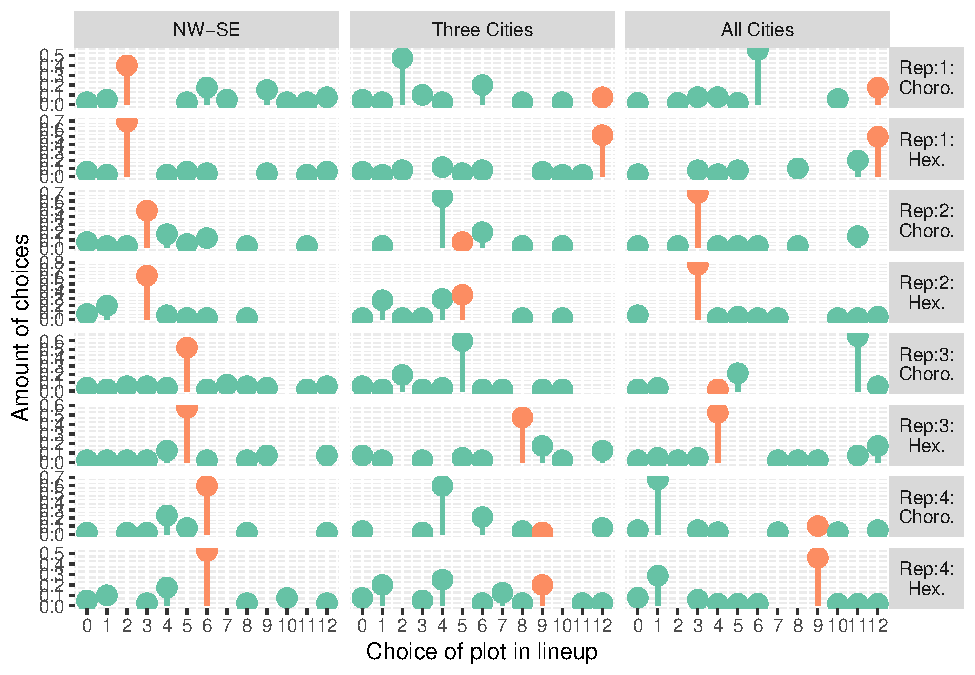
\includegraphics{paper_files/figure-latex/choices-1.pdf}
\caption{Each facet is associated with one lineup, the height of the
points show the proportion of the participants that made each choice
when considering each lineup. The points coloured orange show the map
which contained a trend model, these are the correct choices. The
numbers differentiate the replicates of each trend model and type of map
display. Participants were able to select 0 to indicate they did not
want to choose a map.}
\end{figure}

One lineup had extremely similiar detection rates for the Choropleth and
Hexagon displays.

\begin{figure}
\centering
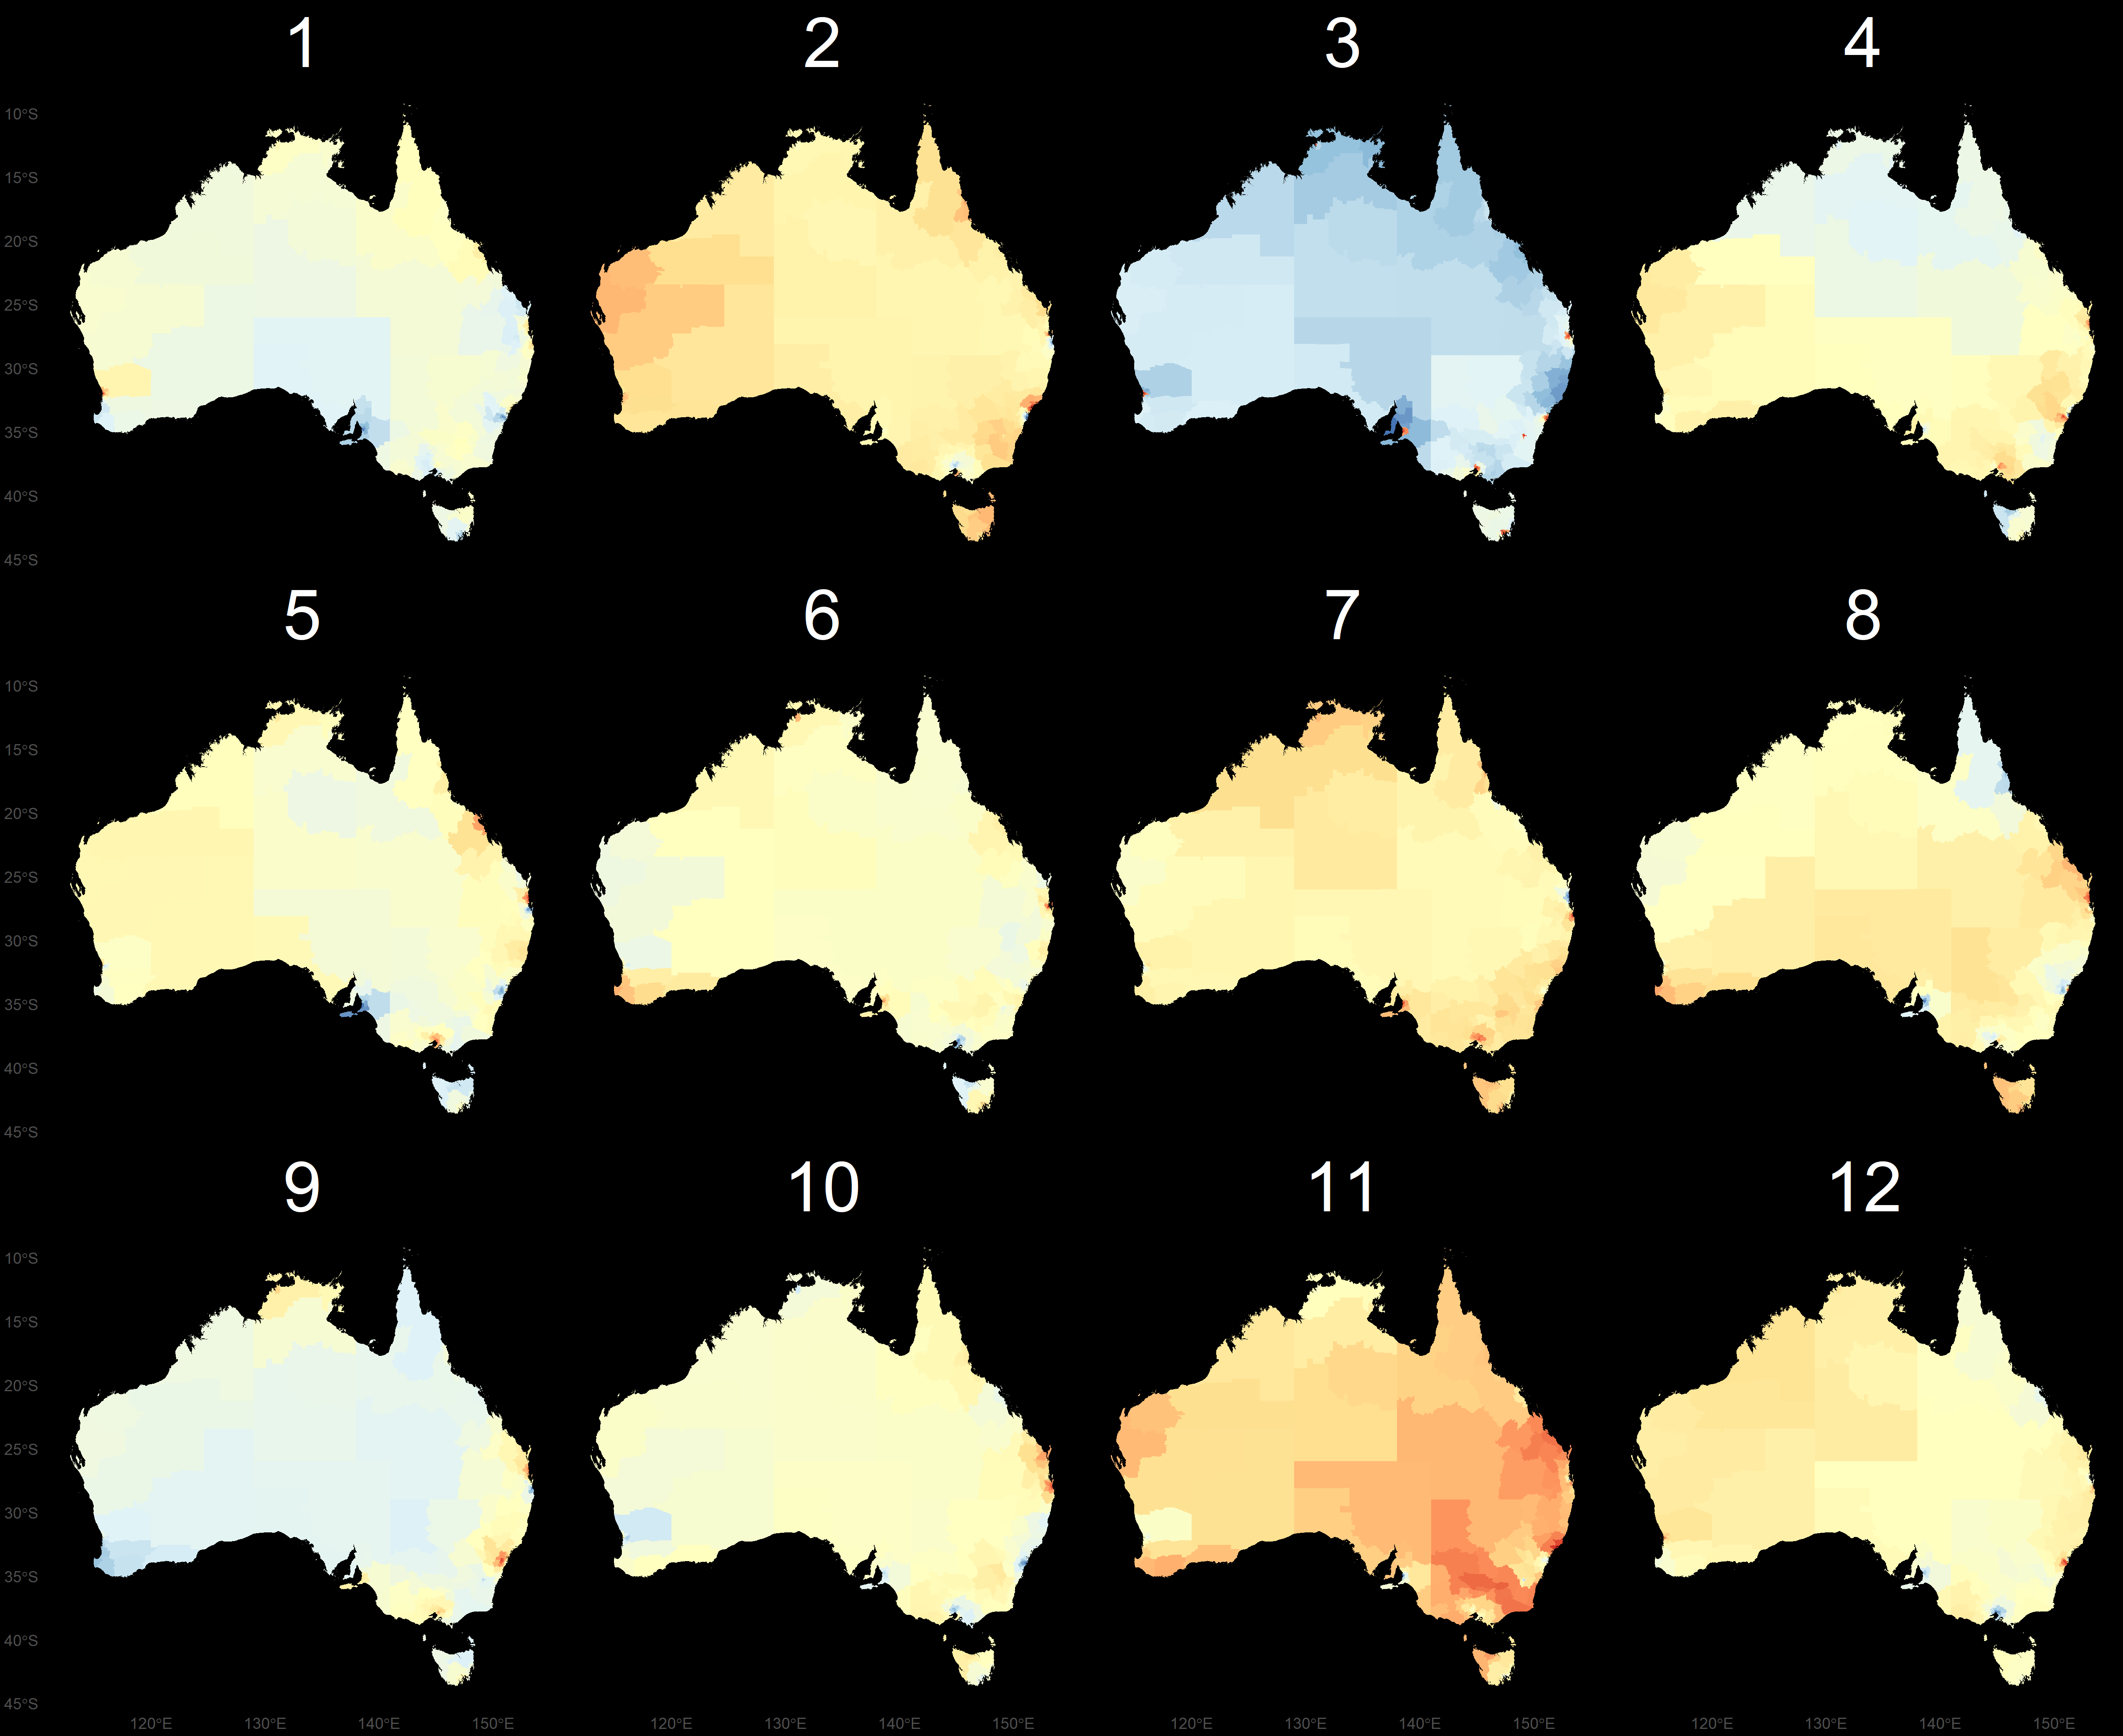
\includegraphics{figures/aus_cities_3_geo.png}
\caption{``The lineup of choropleth map displays shows a distribution
that affects all capital cities. The values for the inner city areas in
the capital cities result in them being coloured red. However, the
colour blue dominates the display as the large rural areas are filled.
Replicate (2) for all cities.''}
\end{figure}

\begin{figure}
\centering
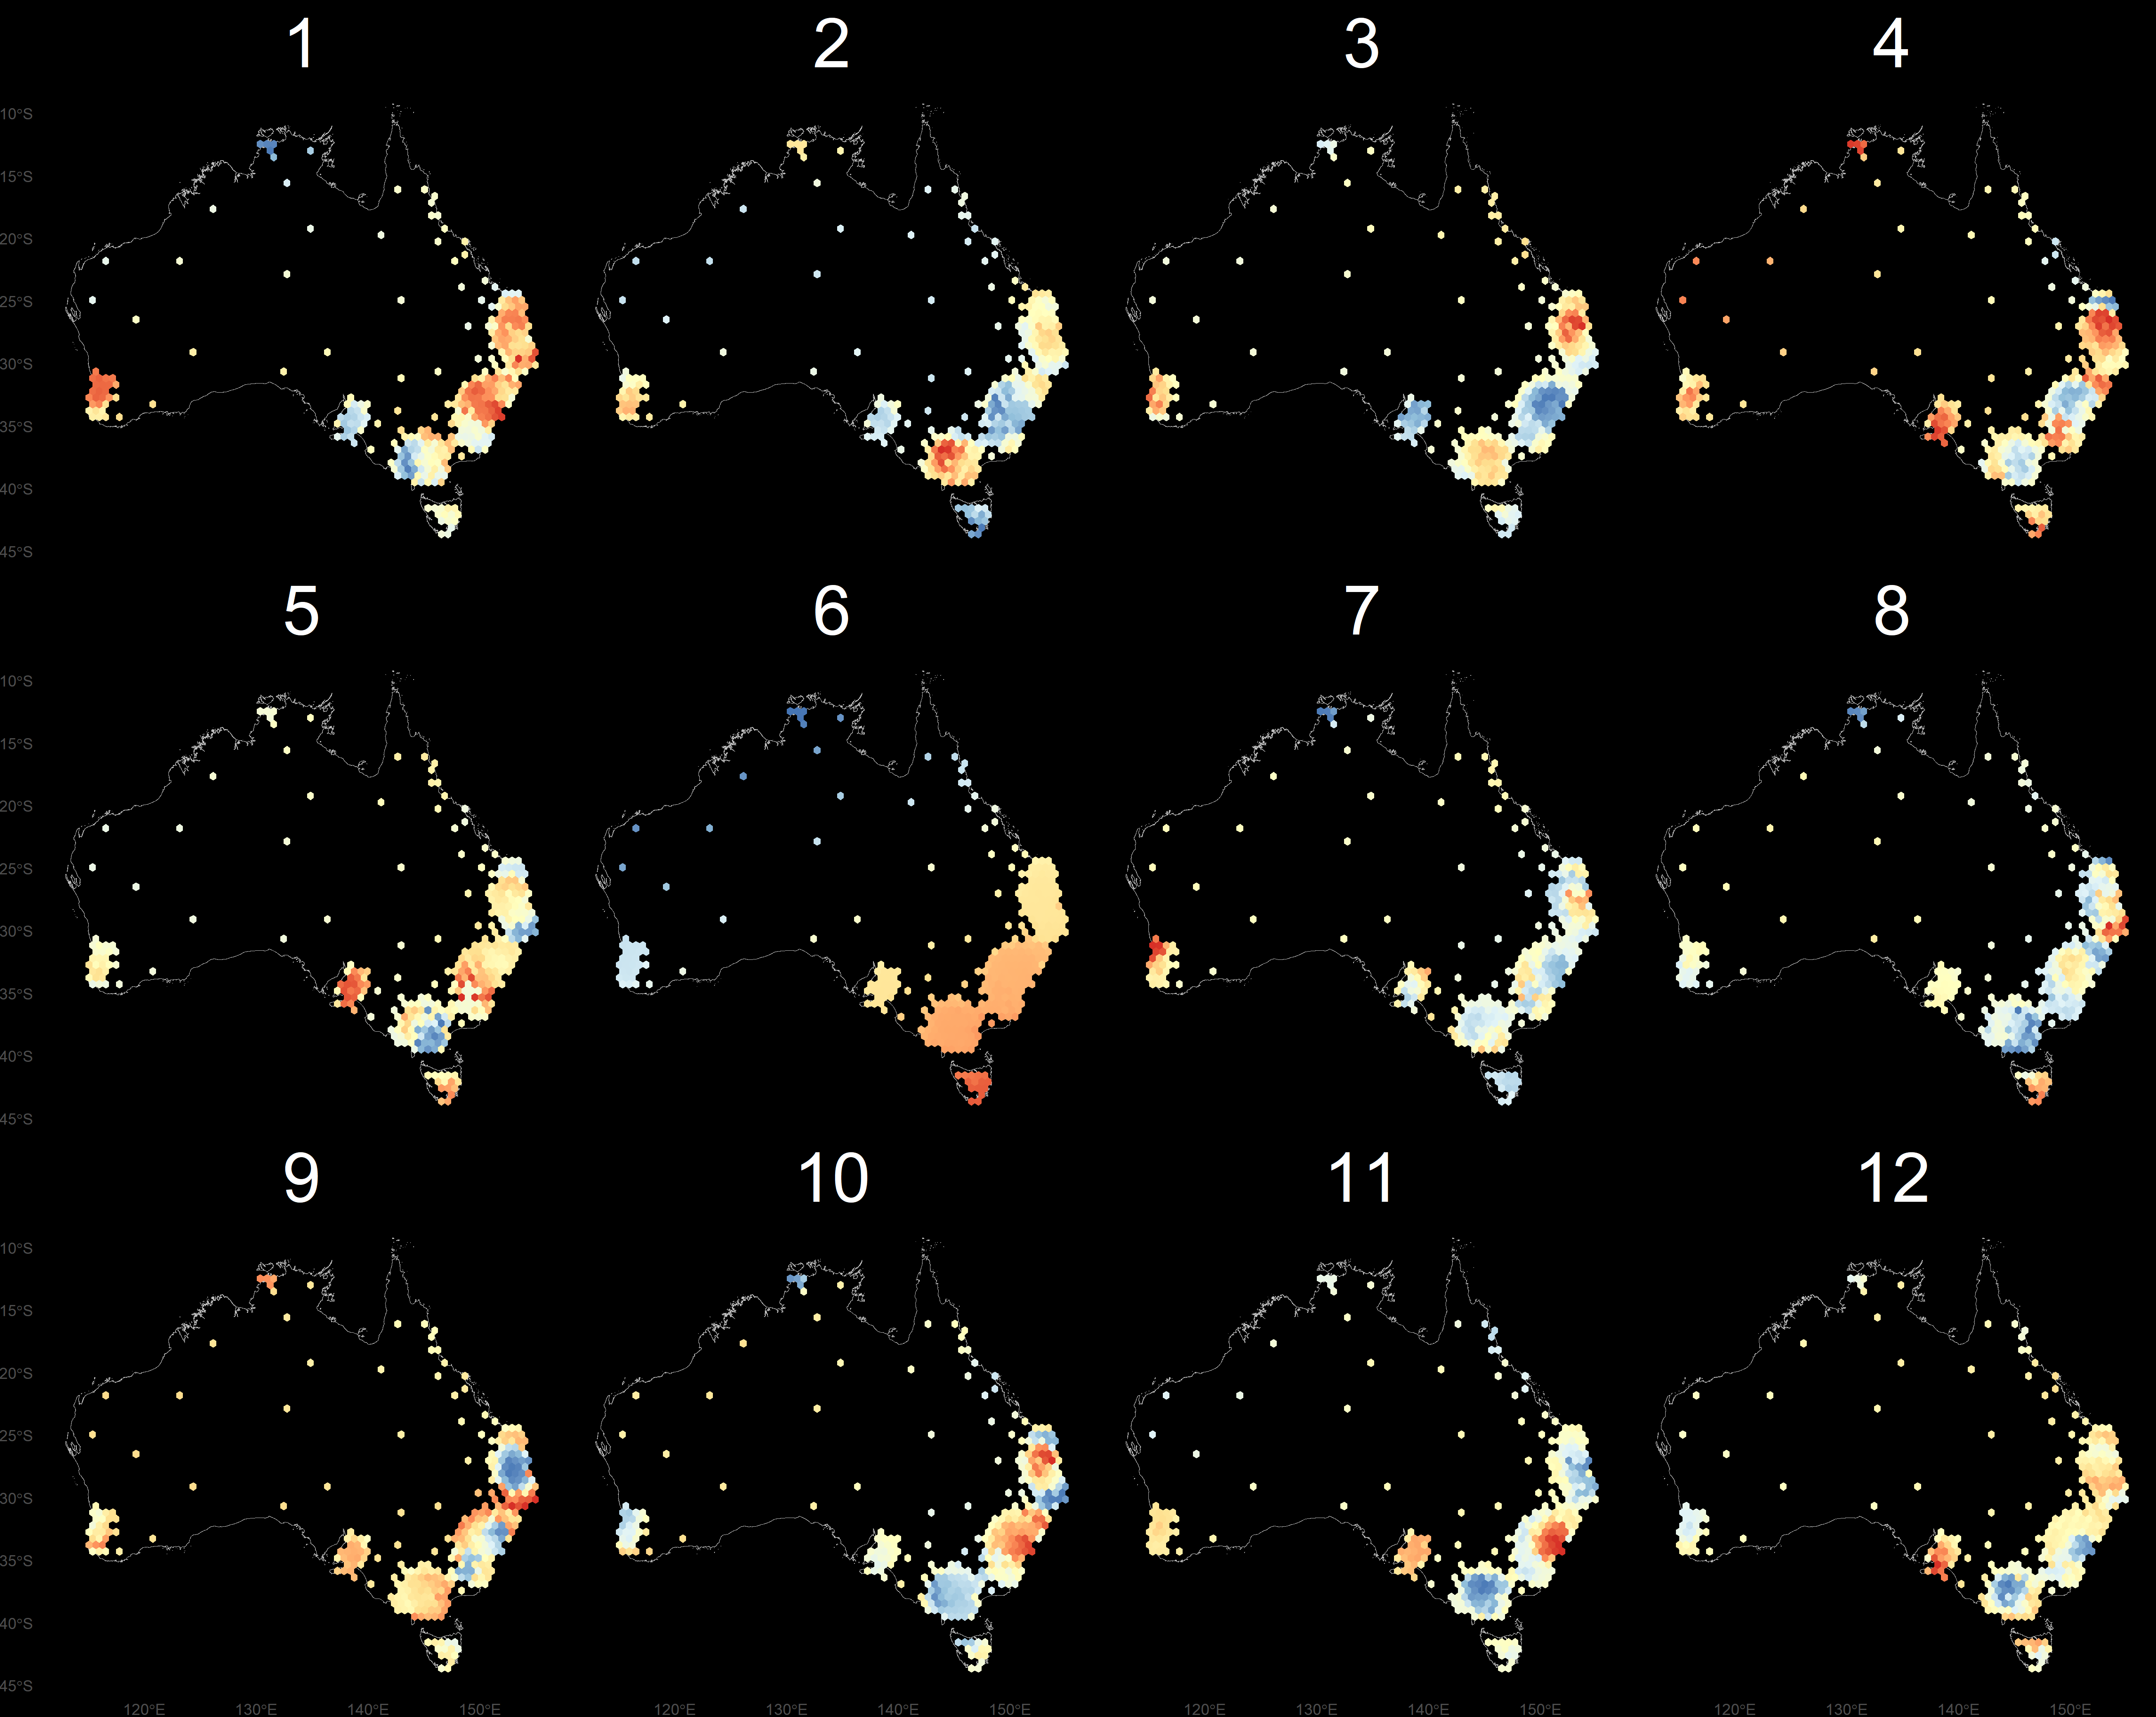
\includegraphics{figures/aus_nwse_6_hex.png}
\caption{``A North-West to South East trend was hidden in this lineup of
hexagon tile map displays.''}
\end{figure}

\hypertarget{modeling-the-difference}{%
\subsection{Modeling the difference}\label{modeling-the-difference}}

The likelihood of detecting the data plot in the lineup can be modelled
using a generalized linear mixed effects model. The base R (R Core Team
\protect\hyperlink{ref-RCore}{2019}) \texttt{glm()} function implements
generalised linear models. The model used includes the two main effects
map type and trend model, which gives the fixed effects model to be:

\[\widehat{y_{ij}} = \mu + \tau_i + \delta_j + (\tau\delta)_{ij} + \epsilon_{i,j}, ~~~ i=1,2; ~j=1,2,3\]

where \(y_{ij} = 0, 1\) whether the subject detected the data plot,
\(\mu\) is the overall mean, \(\tau_i, i=1,2\) is the map type effect,
\(\delta_j\) is the trend model effect. We are allowing for an
interaction between map type and trend model. Because the response is
binary, a logistic model is used. This model can account for each
individual participants' abilities as it includes a subject-specific
random intercept. As each participant provides results from 12 lineups.

\hypertarget{detection-rates}{%
\subsubsection{Detection Rates}\label{detection-rates}}

The model specifies a logistic link, this means the predicted values
from the \texttt{glm} model should be back-transformed to fit between 0
and 1. They are transformed with the link specified below:

\[\mu = \frac{e^{\eta}}{1 + e^{\eta}}\] \[\eta = f(\tau_i,\delta_j)\]

\begin{tabular}{rcrrr}
\toprule
Term & Estimate & Error & Stat & p.value\\
\midrule
Intercept & 0.02 & 0.15 & 0.15 & 0.88\\
Hex & 0.42$^{*  }$ & 0.21 & 1.99 & 0.05\\
Three cities & -3.25$^{***}$ & 0.41 & -7.88 & 0.00\\
All cities & -1.24$^{***}$ & 0.23 & -5.41 & 0.00\\
Hex : Three cities & 2.37$^{***}$ & 0.46 & 5.10 & 0.00\\
\addlinespace
Hex : All cities & 1.08$^{***}$ & 0.31 & 3.47 & 0.00\\
\bottomrule
\end{tabular}

\begin{verbatim}
##                 
##                  Detected? No Detected? Yes
##   Predicted: No           431           121
##   Predicted: Yes          242           310
\end{verbatim}

This gives the model:

\[\widehat{y_{ij}} = 0.0217 + 0.42Hex -3.25_{three} -1.24_{all} + 2.37{Hex.three} + 1.08{Hex.all} \]

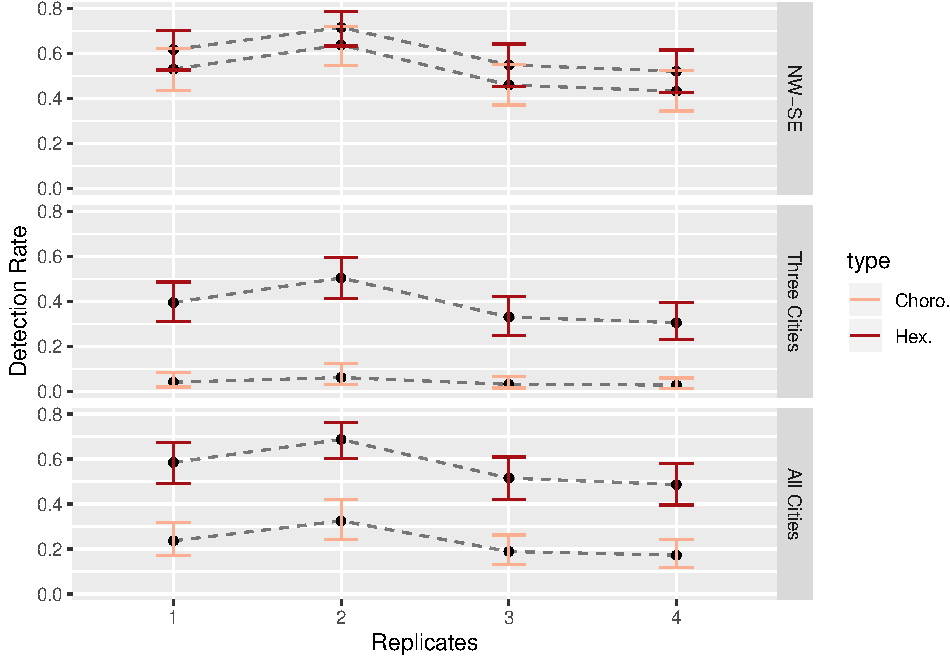
\includegraphics{paper_files/figure-latex/glm2-1.pdf}

\% Table created by stargazer v.5.2.2 by Marek Hlavac, Harvard
University. E-mail: hlavac at fas.harvard.edu \% Date and time: Fri, Jan
10, 2020 - 11:55:55

\begin{table}[!htbp] \centering 
  \caption{} 
  \label{} 
\begin{tabular}{@{\extracolsep{5pt}}lc} 
\\[-1.8ex]\hline 
\hline \\[-1.8ex] 
 & \multicolumn{1}{c}{\textit{Dependent variable:}} \\ 
\cline{2-2} 
\\[-1.8ex] & detect \\ 
\hline \\[-1.8ex] 
 typeHex. & 0.103$^{**}$ \\ 
  & (0.045) \\ 
  & \\ 
 trendThree Cities & $-$0.467$^{***}$ \\ 
  & (0.045) \\ 
  & \\ 
 trendAll Cities & $-$0.277$^{***}$ \\ 
  & (0.045) \\ 
  & \\ 
 typeHex.:trendThree Cities & 0.250$^{***}$ \\ 
  & (0.063) \\ 
  & \\ 
 typeHex.:trendAll Cities & 0.239$^{***}$ \\ 
  & (0.063) \\ 
  & \\ 
 Constant & 0.505$^{***}$ \\ 
  & (0.034) \\ 
  & \\ 
\hline \\[-1.8ex] 
Observations & 1,104 \\ 
Log Likelihood & $-$675.359 \\ 
Akaike Inf. Crit. & 1,366.719 \\ 
Bayesian Inf. Crit. & 1,406.772 \\ 
\hline 
\hline \\[-1.8ex] 
\textit{Note:}  & \multicolumn{1}{r}{$^{*}$p$<$0.1; $^{**}$p$<$0.05; $^{***}$p$<$0.01} \\ 
\end{tabular} 
\end{table}

For a base model of Choropleth map, using a NW-SE trend model. The
detection rate for Hexagon tile maps using a NW-SE trend model changes
the log odds of the detection by 0.42.

\% Table created by stargazer v.5.2.2 by Marek Hlavac, Harvard
University. E-mail: hlavac at fas.harvard.edu \% Date and time: Fri, Jan
10, 2020 - 11:55:55

\begin{table}[!htbp] \centering 
  \caption{} 
  \label{} 
\begin{tabular}{@{\extracolsep{5pt}}lc} 
\\[-1.8ex]\hline 
\hline \\[-1.8ex] 
 & \multicolumn{1}{c}{\textit{Dependent variable:}} \\ 
\cline{2-2} 
\\[-1.8ex] & detect \\ 
\hline \\[-1.8ex] 
 Constant & 0.669$^{***}$ \\ 
  & (0.050) \\ 
  & \\ 
\hline \\[-1.8ex] 
Observations & 1,104 \\ 
Log Likelihood & $-$684.772 \\ 
Akaike Inf. Crit. & 1,379.544 \\ 
Bayesian Inf. Crit. & 1,404.578 \\ 
\hline 
\hline \\[-1.8ex] 
\textit{Note:}  & \multicolumn{1}{r}{$^{*}$p$<$0.1; $^{**}$p$<$0.05; $^{***}$p$<$0.01} \\ 
\end{tabular} 
\end{table}

\hypertarget{certainty-1}{%
\subsubsection{Certainty}\label{certainty-1}}

\% Table created by stargazer v.5.2.2 by Marek Hlavac, Harvard
University. E-mail: hlavac at fas.harvard.edu \% Date and time: Fri, Jan
10, 2020 - 11:55:55

\begin{table}[!htbp] \centering 
  \caption{} 
  \label{} 
\begin{tabular}{@{\extracolsep{5pt}}lccccccc} 
\\[-1.8ex]\hline 
\hline \\[-1.8ex] 
Statistic & \multicolumn{1}{c}{N} & \multicolumn{1}{c}{Mean} & \multicolumn{1}{c}{St. Dev.} & \multicolumn{1}{c}{Min} & \multicolumn{1}{c}{Pctl(25)} & \multicolumn{1}{c}{Pctl(75)} & \multicolumn{1}{c}{Max} \\ 
\hline \\[-1.8ex] 
\hline \\[-1.8ex] 
\end{tabular} 
\end{table}

\hypertarget{discussion}{%
\section{Discussion}\label{discussion}}

\hypertarget{conclusion}{%
\section{Conclusion}\label{conclusion}}

The choropleth map display and the tessellated hexagon tile map have
been contrasted in a visual inference study. The hexagon tile map was
significantly more effective for spotting a real data trend model hidden
in a lineup.

This hexagon tile map display should be considered as a visualisation
method when communicating distributions that relate to the population in
each geographic unit. Cancer Atlas products may benefit from the
opportunity to allow exploration via the traditional choropleth map
method as well as an alternative display. The spatial distributions used
to test these displays were inspired by the real spatially smoothed
estimates of the cancer burden on Australian communities. However, this
technique may be extended to other population related distributions,
such as other diseases.

The increasing population densities of capital cities despite large land
area exaserbates the difference in the smallest and largest communities.
The population density structure of Australia can be considered similar
to that of Canada, New Zealand and many others. Therefore, this display
is not only relevant to Australia, but all nations or population
collections that experience densely populated cities alongside vast
rural expanses.

\hypertarget{supplementary-materials}{%
\section{Supplementary Materials}\label{supplementary-materials}}

\hypertarget{training}{%
\subsection{Training}\label{training}}

The participants were trained using three displays. There were
relatively simple lineups and are shown in Figure XXX.

\hypertarget{survey-application}{%
\subsection{Survey application}\label{survey-application}}

The survey application was hosted on a website external to the
Figure-Eight platform. Following suggestions in the documentation, the
information and training required for a participant to make a decision
was included that survey

The demonstrative images of the \texttt{shinydashboard} web application
display the demographic and consent page in Figure @ref(fig:survey1).

\hypertarget{overall-performance}{%
\subsection{Overall Performance}\label{overall-performance}}

\hypertarget{subject-specific-anomolies-0-detection}{%
\subsection{Subject specific anomolies (0\%
detection)}\label{subject-specific-anomolies-0-detection}}

\hypertarget{demographics}{%
\subsection{Demographics:}\label{demographics}}

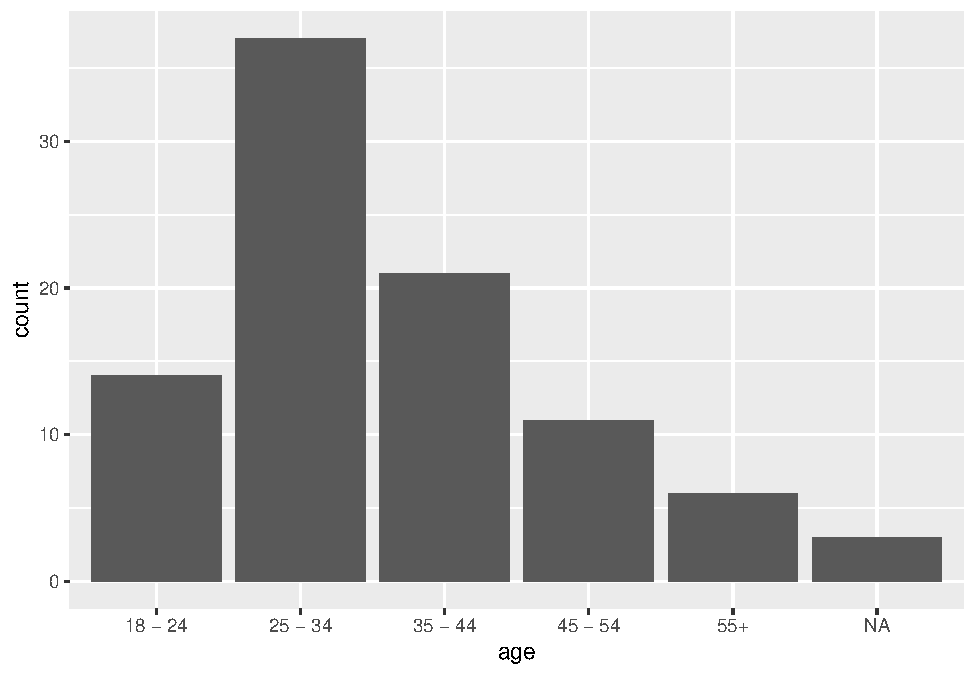
\includegraphics{paper_files/figure-latex/demogs-1.pdf}

\begin{tabular}{lr}
\toprule
gender & n\\
\midrule
He & 67\\
She & 25\\
\bottomrule
\end{tabular}

\begin{tabular}{lr}
\toprule
education & n\\
\midrule
Bach & 56\\
High School & 23\\
Masters & 13\\
\bottomrule
\end{tabular}

\hypertarget{acknowledgment}{%
\section{Acknowledgment}\label{acknowledgment}}

The authors would like to thank\ldots{}

Ethics approval for the online survey was granted by QUT's Ethics
Committee (Ethics Application Number: 1900000991). All applicants
provided informed consent in line with QUT regulations prior to
participating in this research.

\hypertarget{bibliography}{%
\section{Bibliography}\label{bibliography}}

\newpage

\hypertarget{references}{%
\section{References}\label{references}}

\hypertarget{refs}{}
\leavevmode\hypertarget{ref-abs2016}{}%
``Australian Statistical Geography Standard (ASGS).'' 2018.
\emph{Australian Bureau of Statistics}. Australian Government.
\url{\%7Bhttps://www.abs.gov.au/websitedbs/D3310114.nsf/home/Australian\%20\%20\%20Statistical\%20Geography\%20Standard\%20(ASGS)\%7D}.

\leavevmode\hypertarget{ref-lme4}{}%
Bates, Douglas, Martin Mächler, Ben Bolker, and Steve Walker. 2015.
``Fitting Linear Mixed-Effects Models Using lme4.'' \emph{Journal of
Statistical Software} 67 (1): 1--48.
\url{https://doi.org/10.18637/jss.v067.i01}.

\leavevmode\hypertarget{ref-sheets}{}%
Bryan, Jennifer, and Joanna Zhao. 2018. \emph{Googlesheets: Manage
Google Spreadsheets from R}.
\url{https://CRAN.R-project.org/package=googlesheets}.

\leavevmode\hypertarget{ref-GTPCCD}{}%
Hofmann, Heike, Lendie Follett, Mahbubul Majumder, and Dianne Cook.
2012. ``Graphical Tests for Power Comparison of Competing Designs.''
\emph{IEEE Transactions on Visualization and Computer Graphics} 18:
2441--8.

\leavevmode\hypertarget{ref-VVSIALM}{}%
Majumder, Mahbubul, Heike Hofmann, and Dianne Cook. 2013. ``Validation
of Visual Statistical Inference, Applied to Linear Models.''
\emph{Journal of the American Statistical Association} 108 (503):
942--56. \url{https://doi.org/10.1080/01621459.2013.808157}.

\leavevmode\hypertarget{ref-RCore}{}%
R Core Team. 2019. \emph{R: A Language and Environment for Statistical
Computing}. Vienna, Austria: R Foundation for Statistical Computing.
\url{https://www.R-project.org/}.

\leavevmode\hypertarget{ref-GIIV}{}%
Wickham, Hadley, Dianne Cook, Heike Hofmann, and Andreas Buja. 2010.
``Graphical Inference for Infovis.'' \emph{IEEE Transactions on
Visualization and Computer Graphics (Proc. InfoVis '10)} 16 (6):
973--79.

\end{document}


